\documentclass[8pt,landscape]{article}

% PACKAGES
\usepackage[letterpaper, margin=0.1in]{geometry}
\usepackage{amsmath, amssymb, geometry}
\usepackage{multicol}
\usepackage{setspace}
\usepackage{sectsty}
\usepackage{verbatim}
\usepackage{graphicx}
\usepackage{xcolor}
\usepackage{listings}
\usepackage{enumitem}
\usepackage{booktabs} % For better tables if needed

% Define a custom color for code highlighting and environment
\definecolor{myred}{RGB}{204, 0, 0} % A strong red
\definecolor{mygray}{RGB}{240, 240, 240} % Light gray for background
\setlist[itemize]{
    noitemsep,  % Removes vertical space between list items
    topsep=0pt,  % Removes space before the list
    partopsep=0pt, % Removes extra space when a list begins mid-paragraph
    parsep=0pt, % Removes space between paragraphs within an item
    leftmargin=*, % Sets the left margin to the minimum necessary
    labelsep=0.5em, % You can slightly adjust the space between the bullet and the text
}
% LISTINGS SETUP for R and Python
\lstset{
  basicstyle=\ttfamily\scriptsize\color{black},
  backgroundcolor=\color{mygray},
  frame=single,
  frameround=tttt,
  framesep=0pt,        % no padding between code and frame
  rulecolor=\color{black!20},
  rulesep=0pt,         % no space between rules
  breaklines=true,
  columns=fullflexible,
  showstringspaces=false,
  commentstyle=\color{gray},
  keywordstyle=\color{blue!80!black},
  stringstyle=\color{myred},
  breakatwhitespace=true,
  xleftmargin=0pt,     % no left margin
  xrightmargin=0pt,    % no right margin
  aboveskip=0pt,       % no space above listing
  belowskip=0pt,       % no space below listing
  abovecaptionskip=0pt,
  belowcaptionskip=0pt,
  framexleftmargin=0pt,
  framexrightmargin=0pt,
  framextopmargin=0pt,
  framexbottommargin=0pt
}

% FORMATTING
\setstretch{0.9} % Reduce line spacing
\setlength{\parindent}{0pt}
\setlength{\parskip}{0pt}

% Reduce section spacing and change color
\makeatletter
\renewcommand{\section}{\@startsection{section}{2}{0pt}%
    {0.1ex}% space before section
    {0.1ex}% space after section
    {\fontsize{8}{9}\bfseries\color{red}}} % section font: 8pt
\makeatother

% Reduce subsection spacing and make subsections blue
\makeatletter
\renewcommand{\subsection}{\@startsection{subsection}{2}{0pt}%
    {0.1ex}% space before subsection
    {0.1ex}% space after subsection
    {\fontsize{8}{9}\bfseries\color{blue}}} % Subsection font: 8pt
\makeatother

% Custom command for red-highlighted code/commands (for in-line use)
\newcommand{\code}[1]{\textcolor{myred}{\texttt{#1}}}

% Custom small text wrapper - ensuring 8pt for body text
\newcommand{\smalltext}[1]{
  {\fontsize{8}{9}\selectfont\sloppy #1\par}
}

% DOCUMENT START
\begin{document}
\fontsize{8}{9}\selectfont % Set the base font size to 8pt and line skip to 9pt for the entire document
\pagestyle{empty}
\begin{multicols}{3}


\smalltext{
  For simple models, we can sometimes do the math and get a closed-form posterior distribution.
  But in more realistic Bayesian models, especially multi-parameter models, their corresponding posteriors become analytically impossible to write down and manipulate.
\textbf{MCMC} is the simulation approach we use to work around that barrier: instead of deriving the posteriors exactly, we generate approximate posterior samples that behave like draws from the posterior distribution.
 Valid inference for any (finite) amount of data.
  Population parameters of interest are random variables! They have prior and posterior distributions.
  Easy to interpret uncertainty for the population parameters.
  Recursive updating.
}
\smalltext{
  \textbf{Generative Models:}
  A “story about how your data was created.”. Synthetic data (running computational simulations!)

  \textbf{Probabilistic Generative Models:} models incorporate randomness into the system of interest.
  Incorporate noise in measurements. Overly simplified models with incomplete measurements. Incorporate unobservable latent variables.

  \textbf{Rstan:} is a probabilistic C++-based programming language for Bayesian statistical inference 

}

\section{Difference between Probability and Likelihood}
\smalltext{
  Probability and likelihood are NOT the same.
  Probability is the chance of an outcome between 0 to 1. 
  Likelihood is given dataset, which distributional parameter is most likely plausible. Likelihood is not between 0 and 1.
  Probability is MATHEMATICALLY equal to a likelihood, but not STATISTICALLY.
}

\section{Frequentist Drawbacks}
\smalltext{
  We Theoretically Estimate $\pi$ using Maximum likelihood estimation (MLE) is the standard frequentist approach. 
  We cannot incorporate our “expert” intuition, probabilistically speaking.
  How do we use side information, e.g., results of flips from other bottle caps?
  Asymptotic tools tend not to work well with small amounts of data.
  When distributional assumptions break down, the sampling distribution is messy, or the inferential target becomes more complex.
}

\subsection{Definitions of Probability Equation}
\smalltext{
$P(L | T) = \frac{P(L \cap T)}{P(T)}$ 

$P(L | T)$: P of event $L$ occurring given that event $T$ has occurred.

$P(L \cap T)$: P that both event $L$ and event $T$ occur.

$P(T)$: P of the condition, event $T$, occurring on its own.

$\text{new posterior} \propto \text{new likelihood} \times \text{old posterior}$
}

\section{Bayesian Workflow}
\subsection{Likelihood and the "Product Rule" }
\smalltext{
  Bayesians consider the population parameters as random.
  
  When we assume observations are (i.i.d.), the joint likelihood of our data is simply the product of individual probabilities.
  
  \textbf{If Independent:} If you flip a coin 10 times, the likelihood of that sequence is $P(x_1|\theta) \times P(x_2|\theta) \dots \times P(x_{10}|\theta)$. 
  This makes the math easy to compute.
  
  \textbf{If Dependent:} If the outcome of the second flip depends on the first (like drawing cards from a deck without replacement), you cannot just multiply them. You must use conditional probabilities: $P(x_1|\theta) \times P(x_2|x_1, \theta)$.
  
  \textbf{Latent variables } are real but not directly observable quantities, which are linked to what we can measure.
  Instead, we observe partial signals and infer an underlying state.

  \textbf{Recursive Updating} new evidence arrives, we update our beliefs, and yesterday's posterior becomes tomorrow's prior.
  We will update a probability using Bayes' rule, and we will start building the “prior"-"posterior” workflow.

 }
 \subsection{Bayes Rule}
\smalltext{
  The goal of Bayes' Rule is to find the Posterior Probability:
  $P(L | T) = \frac{P(T | L) \cdot P(L)}{P(T)}$ \textbf{Prior:} what we believe before new evidence (e.g., from a previous study).
  \textbf{Evidence term:} how compatible the evidence is with each outcome (e.g., from an observed sample).
  \textbf{Posterior:} what we believe after incorporating the evidence.

  $P(T | L) \neq P(L | T)$. While they use the same variables, they answer fundamentally different questions:
  
  $P(T | L)$ answers: Among people who end up partnered ($L$), how many used Tinder ($T$)?
  
  $P(L | T)$ answers: Among people who used Tinder ($T$), how many end up partnered ($L$)?

  This is Bayesian inference!
  Hidden variables of interest are random (the prior distribution).
  We use the conditional distribution of hidden variables given observations (the posterior distribution) to capture uncertainty.
}
\subsection{MAP and MLE}
\smalltext{
  Maximum a posteriori (MAP) estimation is the Bayesian version of maximum likelihood estimation (MLE).
  MLE aims to find the value that maximizes the sample’s likelihood function (i.e., we are just relying on our observed sampled data!).
  MAP aims to obtain the value that maximizes our posterior distribution, which was obtained with our observed data (i.e., our evidence via the likelihood) weighted by our prior probability model.
}

\section{Bayesian modelling involves these steps:}
\smalltext{

  No p-values in bayesian models, p-value is a frequentist tools.
  As the data become more informative, the likelihood dominates, and the posterior becomes less sensitive to this prior choice.
  It is a big joint probability distribution.

  \textbf{Question:} Pose a scientific question.

  \textbf{Design:} Formulate variables and create a probabilistic model for them. Prior knowledge is included here!

  \textbf{Infer:} Get posterior samples from the conditional distribution of any variable you want to infer, given your observed data and prior knowledge.

  \textbf{Check:} Make sure the “samples” are actually from your posterior (these are model diagnostics, to be covered in week 4!)

  \textbf{Analyze:} Use your samples to compute summaries: mean, maximum a posteriori (MAP), variance, posterior credible intervals (to be explained today), etc.
}

\subsection{The Likelihood Selection (The "Design" Phase)}
\smalltext{
  The first question is: What is the nature of your outcome variable? 
}
\begin{itemize}
  \item \textbf{Binary (Yes/No, Win/Loss)} 
  \\ 
  \textit{Likelihood:} Bernoulli / Binomial 
  \textit{Latent Variable:} Probability of success ($\pi$)
  \textit{Bounds:} $0 \le \pi \le 1$
  \textit{Example:} Did the Cubs win or lose?
  
  \item \textbf{Counts ($0, 1, 2, \dots$)} 
  \textit{Likelihood:} Poisson
  \textit{Latent Variable:} Expected rate ($\lambda$) - continous
  \textit{Bounds:} $\lambda > 0$
  \textit{Example:} How many runs were scored in a game?
  
  \item \textbf{Continuous (No bounds)} 
  \textit{Likelihood:} Normal (Gaussian)
  \textit{Latent Variable:} Mean ($\mu$)
  \textit{Bounds:} $-\infty < \mu < \infty$
  \textit{Example:} What is the average height of a player?
  
  \item \textbf{Continuous (Positive only)} 
  \textit{Likelihood:} Log-Normal / Gamma
  \textit{Latent Variable:} Shape ($\alpha$) and Rate ($\beta$)
  \textit{Bounds:} $\alpha > 0, \beta > 0$
  \textit{Example:} How long is the duration of a game?
  
  \item \textbf{Waiting Times} 
  \textit{Likelihood:} Exponential
  \textit{Latent Variable:} Rate of decay ($\lambda$)
  \textit{Bounds:} $\lambda > 0$
  \textit{Example:} How much time between home runs?
\end{itemize}

\subsection{The Prior Selection (The "Question" Phase)}
\smalltext{
  The prior represents your initial "latent" state (like Team Skill $S_j$).
  
  \textbf{Weakly Informative (The "Peer" Choice): }Use $\text{Normal}(0, 10)$ or $\text{Gamma}(1, 1)$. These say, "I have a guess, but I'm open to being wrong."
  
  \textbf{Conjugate Priors (The "Math Shortcut"):} Choose a prior that "matches" your likelihood so the posterior is in the same family.
  
  Binomial Likelihood $\rightarrow$ Beta Prior
  
  Poisson Likelihood $\rightarrow$ Gamma Prior
  
  Normal Likelihood $\rightarrow$ Normal Prior
}

\subsection{The Inference Method (The "Infer" Phase)}
\smalltext{
  How will you actually calculate the posterior?
  When the prior is from the same family as the posterior, we call it a CONJUGATE PRIOR.
  \textbf{Grid Approximation:} Use only for 1D problems.
  \textbf{Conjugate Math:} Use when you need an instant, exact analytical answer and the model is simple.
  \textbf{MCMC (Stan):} Use for everything else. If you have multiple teams, hierarchical leagues, or complex predictors, you need a sampler like NUTS (No-U-Turn Sampler).
}

\section{Beta-Binomial}
\begin{lstlisting}[language=R]
  data {
    int<lower=1> n;    # Total number of trials
    int<lower=0> X;    # Number of observed successes
    real<lower=0> a;   # Hyperparameter 'alpha' for the Beta prior
    real<lower=0> b;   # Hyperparameter 'beta' for the Beta prior
  } 
  parameters {    
    real<lower=0, upper=1> pi; #Unknown param we want to estimate
  } 
  model {
    pi ~ beta(a, b); # 1. THE PRIOR - gives pi a distribution before seeing the data and params that define it
    X ~ binomial(n, pi); # 2. THE LIKELIHOOD This is the line that tells Stan how the observed data X are generated.
  }
  rocket_dictionary <- list(n = 20, X = 10,a = 1, b = 1)
  posterior_rockets <- sampling( # MCMC method of simulation
    object = rockets_stan,  # 1. The compiled model
    data = rocket_dictionary, # 2. The input data list
    chains = 2,             # 3. Number of independent scouts
    iter = 10000,           # 4. Total steps per scout
    warmup = 1000,          # 5. Learning the terrain (discarded)
    thin = 5,               # 6. Saving every Nth step
    seed = 553,             # 7. Reproducibility key
    algorithm = "NUTS"      # 8. The navigation strategy
  )
  round(qbeta(p = c(0.025, 0.975), shape1 = 42, shape2 = 18), 2)
\end{lstlisting}

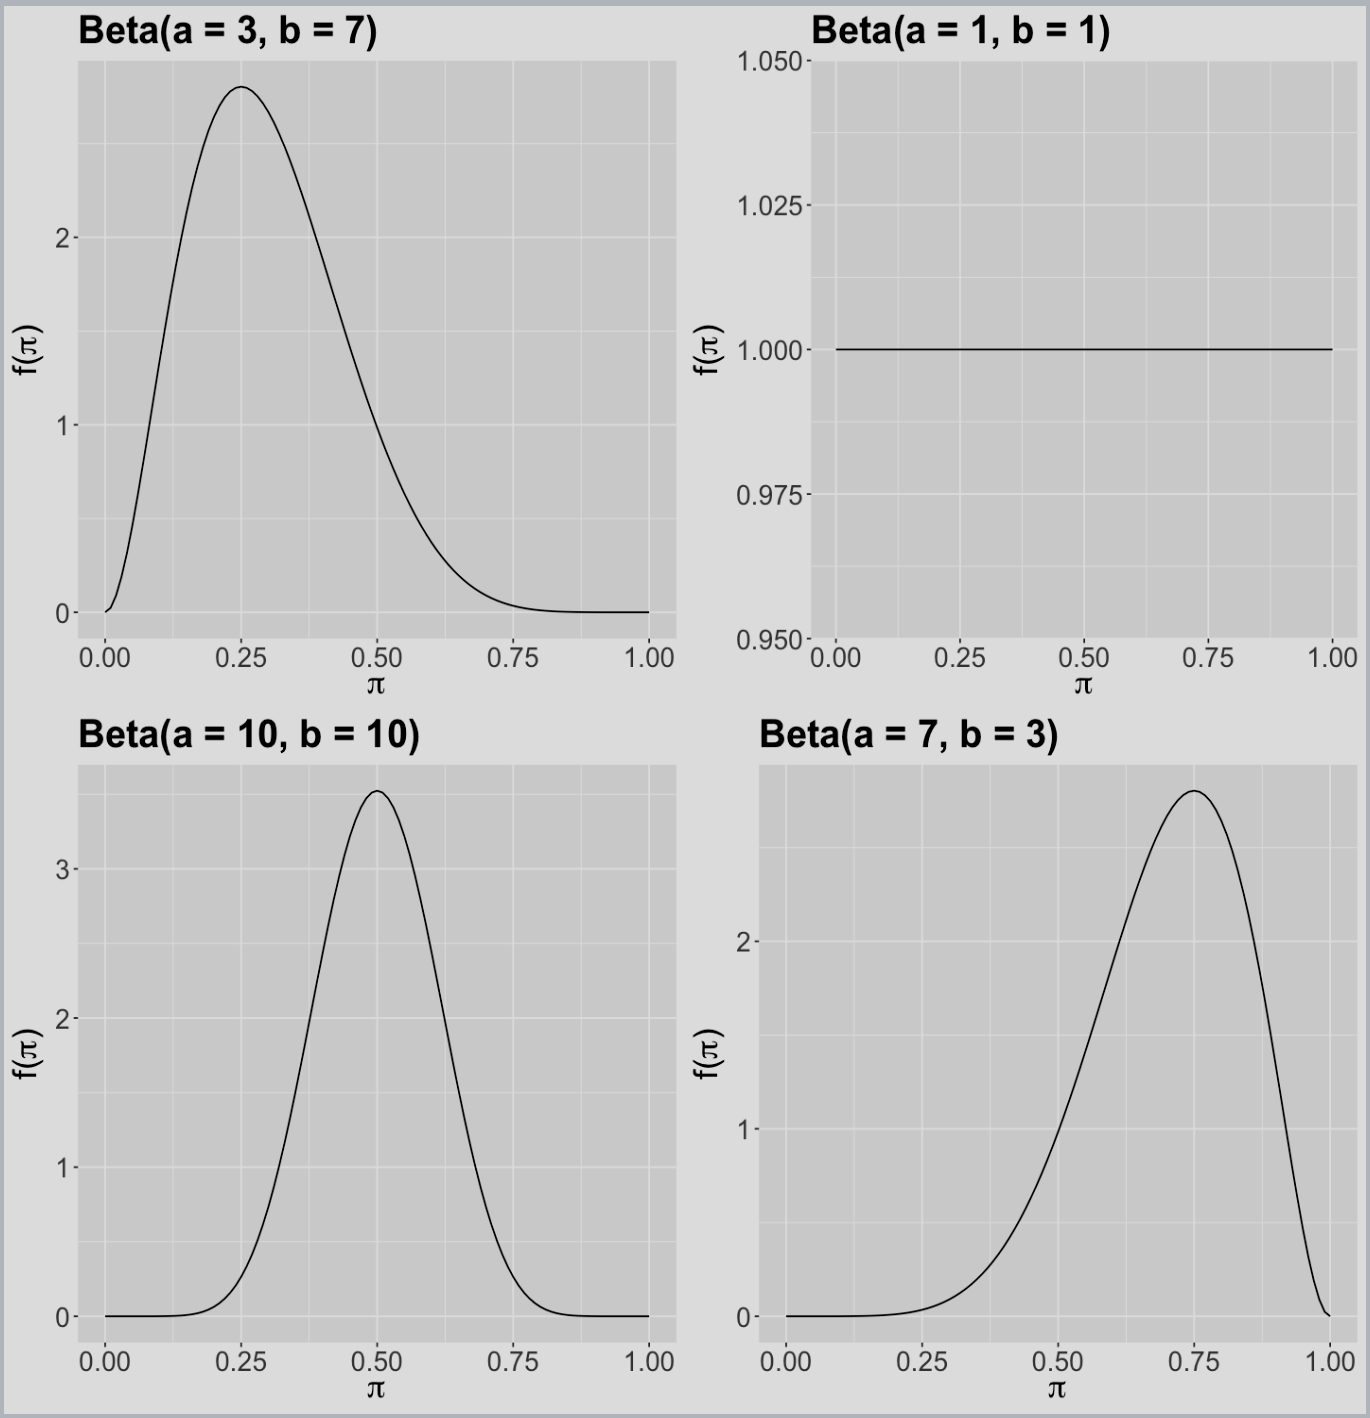
\includegraphics[width=0.5\linewidth, height=2cm]{beta.png}
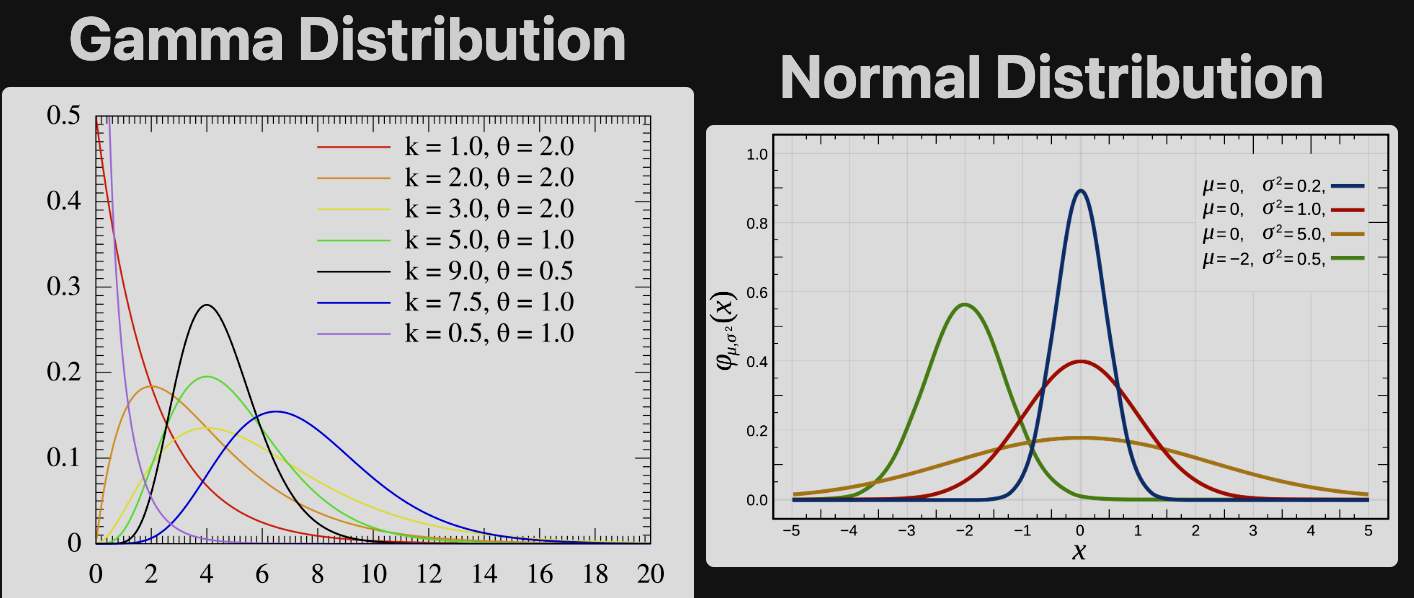
\includegraphics[width=0.5\linewidth, height=2cm]{Gamma.png}

\section{Gamma-Poisson}
\smalltext{
  Therefore, our \textbf{prior distributions} for these weather parameters would be:
$
\begin{aligned}
l_w & \sim \mathcal{N}(\mu, \sigma^2) \quad \text{for} \quad w \in \{1, 2, 3\} \\
a_w & \sim \text{Gamma}(k, \theta) \quad \text{for} \quad w \in \{1, 2, 3\}.
\end{aligned}
$
Now, we have \textbf{hyperparameters}! They are:
    [$\mu, \sigma^2$:] Mean and variance for the Normal distribution.
    [$k, \theta$:] Shape and scale for the Gamma distribution.
}

\section{Monte Carlo Algorithm}
\smalltext{
  We will start with the simple Monte Carlo algorithm. Suppose you have a closed analytical form for the posterior distribution $f(\Theta \mid \mathbf{y})$ (e.g., the Beta posterior in the Beta-Binomial model). You can build your \textbf{independent} Monte Carlo sample $\{\Theta_1, \dots, \Theta_N\}$ of size $N$, from $f(\Theta \mid \mathbf{y})$ by selecting each element $\Theta_i$ ($i = 1, \dots, N$) in the following way:
\textbf{Step 1.} Draw $\Theta_i$ from $f(\Theta \mid \mathbf{y})$.
     \textbf{Step 2.} Go there.  
  This is a random walk!
}

\section{Markov Chain}
\smalltext{
  In terms of our Bayesian modelling for the posterior, it is a sequence $\{\Theta_1, \dots, \Theta_N\}$ of size $N$ whose elements are \textbf{NOT ENTIRELY INDEPENDENT} (hence the word chain!).

\textbf{What does NOT ENTIRELY INDEPENDENT implicate?} It implicates the so-called \textbf{Markov property}:

    \textit{The next sampled $\Theta_{i+1}$ will depend on the current $\Theta_i$ but not on previous $\Theta_{i-1}, \Theta_{i-2}, \dots$}
More formally, because of this property, the conditional probability function of $\Theta_{i+1}$ can be depicted as:
$f(\Theta_{i+1} \mid \Theta_i, \mathbf{y}) = f(\Theta_{i+1} \mid \Theta_1, \Theta_2, \dots, \Theta_i, \mathbf{y}).$
}

\section{The Metropolis-Hastings Algorithm}
\smalltext{
  This algorithm allows us to obtain an \textbf{approximation of the posterior distribution} $f(\Theta \mid \mathbf{y})$ via our Markov Chain $\{\Theta_1, \dots, \Theta_N\}$.

  Recall Bayes' rule:
 $ f(\Theta \mid \mathbf{y}) \propto f(\Theta) \times \ell(\Theta \mid \mathbf{y}). $
  
  Let the current $\Theta_i = \Theta$. The algorithm's two steps are:
   \textbf{Step 1.} Randomly draw a new location $\Theta'$ from a proposed model with PDF $q(\Theta' \mid \Theta)$. This is a \textbf{jumping distribution} (e.g., symmetric \textbf{Uniform} or \textbf{Normal}, or asymmetric \textbf{Log-normal} for non-negative constraints).
   \textbf{Step 2.} Decide whether to ``go'' or ``not to go'' to the proposed $\Theta'$.
}

\section{MCMC}
\smalltext{
  The approximate posterior's width is determined by the model (our likelihood and any
  noise/variability assumptions), the prior (how concentrated your beliefs are before seeing data), and the
  observed data (how much information the data contain, often more observations or less noisy measurements
  make the likelihood more concentrated). In contrast, MCMC settings like warmup length, iterations, and
  number of chains do not change the target posterior; they mainly affect whether the chains explore it
  adequately and whether the resulting posterior summaries and plots are stable and trustworthy
}





% 
\includegraphics[width=0.5\linewidth, height=2cm]{silllo.png}
% 
\includegraphics[width=0.5\linewidth, height=2cm]{silllo-2.png}


\end{multicols}
\end{document}
